\documentclass[12pt]{article}
\usepackage{geometry} % Pour passer au format A4
\geometry{hmargin=1cm, vmargin=1cm} % 

% Page et encodage
\usepackage[T1]{fontenc} % Use 8-bit encoding that has 256 glyphs
\usepackage[english,french]{babel} % Français et anglais
\usepackage[utf8]{inputenc} 

\usepackage{lmodern}
\setlength\parindent{0pt}

% Graphiques
\usepackage{graphicx,float,grffile}

% Maths et divers
\usepackage{amsmath,amsfonts,amssymb,amsthm,verbatim}
\usepackage{multicol,enumitem,url,eurosym,gensymb}

% Sections
\usepackage{sectsty} % Allows customizing section commands
\allsectionsfont{\centering \normalfont\scshape}

% Tête et pied de page

\usepackage{fancyhdr} 
\pagestyle{fancyplain} 

\fancyhead{} % No page header
\fancyfoot{}

\renewcommand{\headrulewidth}{0pt} % Remove header underlines
\renewcommand{\footrulewidth}{0pt} % Remove footer underlines

\newcommand{\horrule}[1]{\rule{\linewidth}{#1}} % Create horizontal rule command with 1 argument of height

%----------------------------------------------------------------------------------------
%   Début du document
%----------------------------------------------------------------------------------------

\begin{document}

%----------------------------------------------------------------------------------------
% RE-DEFINITION
%----------------------------------------------------------------------------------------
% MATHS
%-----------

\newtheorem{Definition}{Définition}
\newtheorem{Theorem}{Théorème}
\newtheorem{Proposition}{Propriété}

% MATHS
%-----------
\renewcommand{\labelitemi}{$\bullet$}
\renewcommand{\labelitemii}{$\circ$}
%----------------------------------------------------------------------------------------
%   Titre
%----------------------------------------------------------------------------------------

\setlength{\columnseprule}{1pt}

\horrule{2px}
\section*{Chapitre 3 - Puissances}
\horrule{2px}

\section*{1 - L'opération puissance}


  \subsection*{Les puissances positives}
  
  \textbf{L'opération puissance est une nouvelle opération}. On multiplie un nombre par lui-même un certain nombre de fois. En ce point, elle ressemble à la multiplication. \textit{On lit deux puissance quatre}. 

  \begin{flalign*}
    2 + 2 + 2 + 2 &= 2 \times 4 \\
    2 \times 2 \times 2 \times 2 &= 2^4 \\
  \end{flalign*}

Quelques exemples : 

  \begin{flalign*}
    5^6  &= 5 \times 5 \times 5 \times 5 \times 5 \times 5 \\
    (-3)^4  &= -3 \times -3 \times -3 \times -3 
  \end{flalign*}
  
  \textit{Il va falloir être prudent sur les priorités de calculs. (voir exercices)}
  
  \subsection*{Les puissances de 2 négatives}

  L'opération puissance fonctionne aussi avec des \textbf{exposants négatifs}. On multiplie alors un certain nombre de fois par l'inverse du nombre de départ. 

  \begin{flalign*}
    2^{-4} &= \dfrac{1}{2} \times \dfrac{1}{2} \times \dfrac{1}{2} \times \dfrac{1}{2} = \dfrac{1}{ 2 \times 2 \times 2 \times 2} = \dfrac{1}{2^4}
  \end{flalign*}

  \subsection*{Les puissances de 2}

  Les puissances de 2 sont utilisées à la base de l'informatique pour stocker des nombres en mémoire dans le système de numération binaire.

  \begin{flalign*}
   2^1 &= 2 \\
   2^2 &= 4 \\
   2^3 &= 8 \\
   2^4 &= 16 \\
   2^5 &= 32 \\
   2^6 &= 64 \\
   2^7 &= 128 \\
   2^8 &= 256 \\
   2^9 &= 512 \\
   2^{10} &= 1024 \\
  \end{flalign*}

\newpage

\section*{2 - La notation scientifique}

\subsection*{Les grands nombres}

\begin{multicols}{2}

  L'opération puissance permet d'obtenir rapidement de très grands nombres.

  $$2^{64} = 18 \, 446 \, 744 \, 073 \, 709 \, 551 \, 616$$

  \paragraph{Problème :}

  \begin{itemize}
  \item Ce nombre est difficile à lire.
  \item Ce nombre est long à représenter.
  \item Ce nombre est source d'erreur à écrire.
  \end{itemize}

  Les calculatrices présentent les résultats autrement : \textbf{la forme scientifique.}

  $$2^{64} = 1,844 \, 674 \, 407 \times 10^{19}$$

  \underline{Pour écrire un nombre sous forme scientifique :} \\
  \begin{itemize}
  \item on place la virgule après le premier chiffre puis on multiplie par une puissance de 10. \\
  \end{itemize}

  La puissance de 10 s'appelle \textbf{l'ordre de grandeur.}\\
  \textit{On le lit : un virgule quatre-vingt-quatre fois dix puissance dix-neuf.}

  \paragraph{Conclusion :}

  \begin{itemize}
  \item La représentation de ce nombre tient à l'écran.
  \item Ce nombre est facile à lire et à écrire.
  \item On comprend tout de suite l'ordre de grandeur de ce nombre.
  \end{itemize}

    \textbf{La notation scientifique} utilise les puissances de dix. Pour connaître l'ordre de grandeur, on compte le nombre de chiffre entre le premier chiffre et le chiffre des unités. \\ 

\end{multicols}
\subsection*{Les petits nombres}
\begin{multicols}{2}



  On rencontre les mêmes problèmes avec les petits nombres.

  $$2^{-10} = 0, 000 \, 976\, 562\, 5$$

  Pour les mêmes raisons, les calculatrices vont aussi les représenter sous \textbf{forme scientifique}.

  $$2^{-10} = 9, 7654 \, 625 \times 10^{-4}$$

  \textit{On le lit : neuf virgule soixante seize fois dix puissance moins quatre.} \\
  \textbf{La notation scientifique} utilise les puissances de dix négatives pour représenter les petits nombres. Afin de connaître l'ordre de grandeur, on compte le nombre de 0 en partant du premier. \\

\end{multicols}
  \subsection*{Les puissances de 10}
\begin{multicols}{2}

  \underline{Liste des premières puissances de 10 :} 

  \begin{itemize}
  \item $10^0 = 1 $ // Par définition 
  \item $10^1 = 10$ // On multiplie par dix.
  \item $10^2 = 100$ // On multiplie par cent.
  \item $10^3 = 1 \, 000$ // On multiplie par mille.
  \item $10^4 = 10 \, 000$ // On multiplie par dix mille.
  \item $10^5 = 100 \, 000$ // On multiplie par cent mille.
  \item $10^6 = 1 \, 000\, 000$ // On multiplie par un million.
  \item $10^9 = 1 \, 000\, 000 \, 000$ 
  \item $10^{12} =1 \, 000 \, 000 \, 000 \, 000$
  \end{itemize}

  \underline{Liste des premières puissances de 10 négatives:} 

  \begin{itemize}
  \item $10^0 = 1 $ // Par définition 
  \item $10^{-1} = 0,1$ // On multiplie par un dixième.
  \item $10^{-2} = 0,01$ // On multiplie par centième.
  \item $10^{-3} = 0,001$ // On multiplie par un millième.
  \item $10^{-4} = 0,000 \, 1$ 
  \item $10^{-5} = 0,000 \, 01$ 
  \item $10^{-6} = 0,000 \, 001$ .
  \item $10^{-9} = 0,000 \, 000 \, 000 \, 1$ 
  \end{itemize}
\end{multicols}

\newpage

\section*{3 - Trucs et astuces}

Il existe \textbf{des règles} pour simplifier \textit{à la main} les puissances dans les calculs. Il faudra être prudent avec les puissances négatives et faire attention aux signes. Le but n'est pas de calculer mais de proposer une écriture plus simple.

\setlength{\columnseprule}{0pt}

\begin{multicols}{2}
  \begin{itemize}
  \item \textbf{Règle 1 : } $ 2^{10} \times 2^{12} = 2^{10 + 12} = 2^{22} $
  \item \textbf{Règle 2 : } $ \dfrac{14^{25}}{14^{10}} = 14^{25 - 10} = 14^{15} $  
  \item \textbf{Règle 3 : } $ (10^4)^9 = 10^{4 \times 9} = 10^36 $
  \item \textbf{Règle 4 : } $ 5^{19} \times 7^{19} = (5 \times 7)^{19} = 35^{19} $
    \end{itemize}
\end{multicols}

\section*{4 - La science et le numérique}

Très rapidement, ce chapitre permet d'atteindre et de comprendre les limites de notre calculatrice. \\

\subsection*{Les pièges à la calculatrice}

  \begin{itemize}
  \item $10^{12} + 1 = 10^{12} $. La calculatrice calcule \textbf{just}e mais nous affiche \textbf{faux}. La preuve étant que $10^12 + 1 - 10^12 = 1$ à la calculatrice.
  \item $10^{14} + 1 = 10^{14} $. La calculatrice calcule \textbf{faux} et nous affiche \textbf{faux}. La preuve étant que $10^14 + 1 - 10^14 = 0$ ce qui est faux... On peut avoir le bon résultat en changeant l'ordre des calculs : $10^14 - 10^14 +1 = 1$ 
  \item $\dfrac{10^{100}}{10^{100}} = \text{ERREUR !} $. Notre calculaltrice ne sait calculer pas avec des nombres aussi grand et nous le dit... même si le résultat est petit..
  \end{itemize}

\subsubsection*{En quête du sens physique : le très grand}

\begin{multicols}{2}

  \begin{figure}[H]
        \centering
        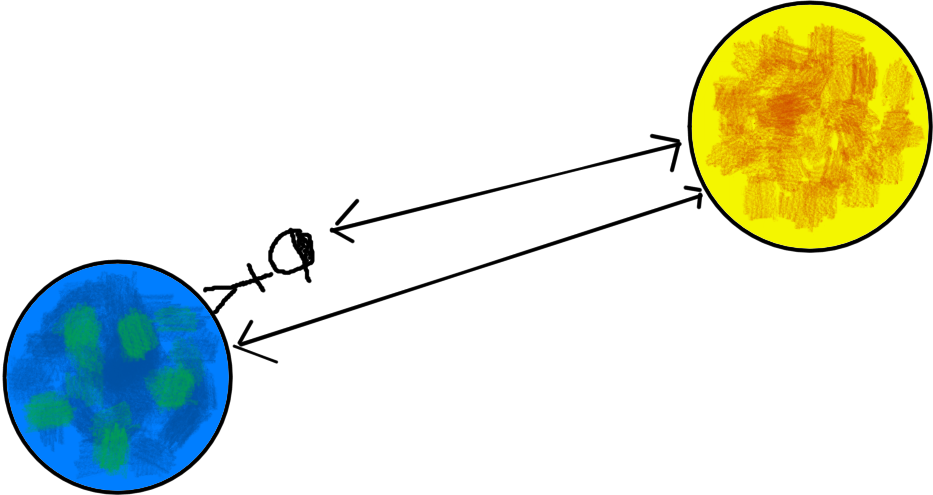
\includegraphics[width=0.8\linewidth]{4x3-puissances/sources/terre.png}
  \end{figure}

  \begin{flalign*}
        10^{16} - 10^{16} + 1,6 &= 1,6 \\
        10^{16} + 1,2 - 10^{16} &= 0 \text{\textbf{ !!!}}
  \end{flalign*}

  Pour nos calculatrices : $10^{16} + 1,6 = 10^{16}$. \\
  Scientifiquement, l'\textbf{approximation} est acceptable. \\
  La distance Terre-Soleil est la même que l'on mesure de notre tête ou de nos pieds.

\end{multicols}

\subsubsection*{En quête du sens physique : le très petit}

\begin{multicols}{2}

  \begin{figure}[H]
        \centering
        
\includegraphics[width=0.8\linewidth]{4x3-puissances/sources/papier.png}
  \end{figure}

  \begin{flalign*}
        12,5 - 12,5 + 10^{-16} &= 10^{-16} \\
        12,5 + 10^{-16} - 12,5 &= 0 \text{\textbf{ !!!}}
  \end{flalign*}

  Pour nos calculatrices : $10^{-16} + 1,6 = 1,6$.\\
  Scientifiquement, l'\textbf{approximation} est acceptable.\\
  Je mesure la même taille si je me mesure du sol ou si je marche sur une feuille de papier.
\end{multicols}

\end{document}
